
%% bare_conf.tex
%% V1.4b
%% 2015/08/26
%% by Michael Shell
%% See:
%% http://www.michaelshell.org/
%% for current contact information.
%%
%% This is a skeleton file demonstrating the use of IEEEtran.cls
%% (requires IEEEtran.cls version 1.8b or later) with an IEEE
%% conference paper.
%%
%% Support sites:
%% http://www.michaelshell.org/tex/ieeetran/
%% http://www.ctan.org/pkg/ieeetran
%% and
%% http://www.ieee.org/

%%*************************************************************************
%% Legal Notice:
%% This code is offered as-is without any warranty either expressed or
%% implied; without even the implied warranty of MERCHANTABILITY or
%% FITNESS FOR A PARTICULAR PURPOSE! 
%% User assumes all risk.
%% In no event shall the IEEE or any contributor to this code be liable for
%% any damages or losses, including, but not limited to, incidental,
%% consequential, or any other damages, resulting from the use or misuse
%% of any information contained here.
%%
%% All comments are the opinions of their respective authors and are not
%% necessarily endorsed by the IEEE.
%%
%% This work is distributed under the LaTeX Project Public License (LPPL)
%% ( http://www.latex-project.org/ ) version 1.3, and may be freely used,
%% distributed and modified. A copy of the LPPL, version 1.3, is included
%% in the base LaTeX documentation of all distributions of LaTeX released
%% 2003/12/01 or later.
%% Retain all contribution notices and credits.
%% ** Modified files should be clearly indicated as such, including  **
%% ** renaming them and changing author support contact information. **
%%*************************************************************************


% *** Authors should verify (and, if needed, correct) their LaTeX system  ***
% *** with the testflow diagnostic prior to trusting their LaTeX platform ***
% *** with production work. The IEEE's font choices and paper sizes can   ***
% *** trigger bugs that do not appear when using other class files.       ***                          ***
% The testflow support page is at:
% http://www.michaelshell.org/tex/testflow/



\documentclass[conference]{IEEEtran}

\usepackage{graphicx}
\usepackage{amsmath}
\usepackage{amssymb}
\usepackage{gensymb}

\graphicspath{ {C:/Users/Marc/Documents/Uni/van2016} }

\hyphenation{op-tical net-works semi-conduc-tor}


\begin{document}

\title{Application and Verbalization of Fuzzy Cognitive Maps in the Case of Flight Passenger Flows}

\author{\IEEEauthorblockN{Marc Osswald}
\IEEEauthorblockA{Swiss International Air Lines Ltd.\\
Basel, CH\\
Email: marc.osswald@swiss.com}
\and
\IEEEauthorblockN{Marcel Wehrle}
\IEEEauthorblockA{University of Fribourg\\
Fribourg, CH\\
Email: marcel.wehrle@unifr.ch}
\and
\IEEEauthorblockN{Edy Portmann}
\IEEEauthorblockA{University of Bern\\
Bern, CH\\
Email: edy.portmann@iwi.unibe.ch}}

\maketitle

\begin{abstract}
Fuzzy Cognitive Maps (FCM) are a representation of concepts affecting one another. By connecting these concepts, FCM's are capable to show dependencies and relationships to a certain degree between these.  Normally this dependencies are numerically translated which impedes the interpretability for humans. This paper seeks to turn the mathematical output of a FCM into natural language sentences applying the Restriction Centered Theory (RCT) to enhance the knowledge transfer possibilites of FCM for humans. The proposed framework connects these concepts to produce not only verbalized dependencies but provides also statements about these dependencies of the FCM. As a proof of concept a use case is introduced, where an airline's connecting passenger flows are analyzed. The statements of the frameworks output is verified by an expert of the data-owning company.\\
Keywords: Fuzzy Cognitive Maps, Restriction Centered Theory, Verbalization of dependencies
\end{abstract}

	
\IEEEpeerreviewmaketitle

\section{Introduction}
Dealing with language is simple and complicated at the same time. There is a set of rules stating how words have to be arranged in order to build grammatically correct sentences. By learning and following the rules, one is able to speak the language correctly -- in terms of grammar. The big challenge of using a language is to find exactly those words that express what someone wants to communicate to its counterpart. But it is not guaranteed yet that the listener will interpret these words in the same way as the speaker does. Rapaport \cite{Rapaport2003} states that communication is a negotiation of meanings. If two people do not have a common understanding of the concept behind a word, they will experience a misunderstanding.\\
For computers, the meaning of a sentence cannot be recognized unless he is taught by a human to do so. There are many ways to convert complex information into bits and bytes. But information are supposed to flow also in the other direction. Computers need to be more and more able to decide by themselves, which part of the information is relevant and which one is not. Moreover they need to set information into the right context. By communicating their findings to a human, not only in digits, but in complete sentences (i.e. natural language), the transfer of knowledge is simplified. The computer incurs to some part the interpretation of the numerical expressions.\\
These sentences should be filled with meaningful words. Statements like \emph{"In the past three years, the maximum temperature on Easter Sunday was (5.1\degree C, 6.2\degree C, 2.3\degree C)"} are then replaced by \emph{"In the past three years, Easter Sunday was always a cold day"}. At the same time, the problem of subjectivity raises, if someone thinks that every temperature above 0\degree C does not deserve the linguistic label \emph{"cold"}, then he might be misled by the information. Even worse, if someone has its limit at 5\degree C, then even the word \emph{"always"} is not correct anymore.\\
This kind of difference in interpretation of words is an unsolved problem for computers. But there are a ways to avoid this strict allocation of content to a concept (i.e. fuzzy computation). It allows that absolute values like temperatures may belong not only to a single, but to different concepts.\\
After having introduced the concepts of FCM and RCT in Chapter \ref{sec:theory}, this paper seeks to find a way to shape FCM's out of large data amounts and to phrase the contents into complete and meaningful sentences. To do so, a framework is presented (Chapter \ref{sec:framework}) and implement in a use case (Chapter \ref{sec:usecase}). In the end, Chapter \ref{sec:lessons} presents the lessons learned from the use case, and Chapter \ref{sec:conclusion} features a general conclusion.\\


\section{Theory of FCM and RCT}
\label{sec:theory}
This chapter will present the theoretical elements of the FCM (Section \ref{subsec:fcm}) and the RCT (Section \ref{subsec:rct}).
\subsection{Fuzzy Cognitive Maps}
\label{subsec:fcm}

FCM are an extension of the concept of cognitive maps where precise or abstract concepts can be interconnected \cite{kosko1986}. In cognitive maps the concepts are represented by nodes, the interconnections by directed graphs. Additionally the edges are used for representing the information of how a concept influences another. This information is reduced to a plus or minus, meaning that a concept exerts a positive or a negative influence to its counterpart.\\
Compared to cognitive maps, FCM are capable to give statements about \emph{how much} concepts influence each other by introducing edge weights in the interval between -1 and 1. This leads to a major flexibility and accuracy to represent complex systems.\\
According to Stach et al. \cite{stach2005}, a FCM can be developed either manually or computationally. To visualize the basic idea of a FCM, Figure 1 shows a fictional minimized FCM of how much the profit of a flight route from A to B is being influenced by the number of passengers, the petrol price or the number of connecting passengers.

\begin{figure}[ht]
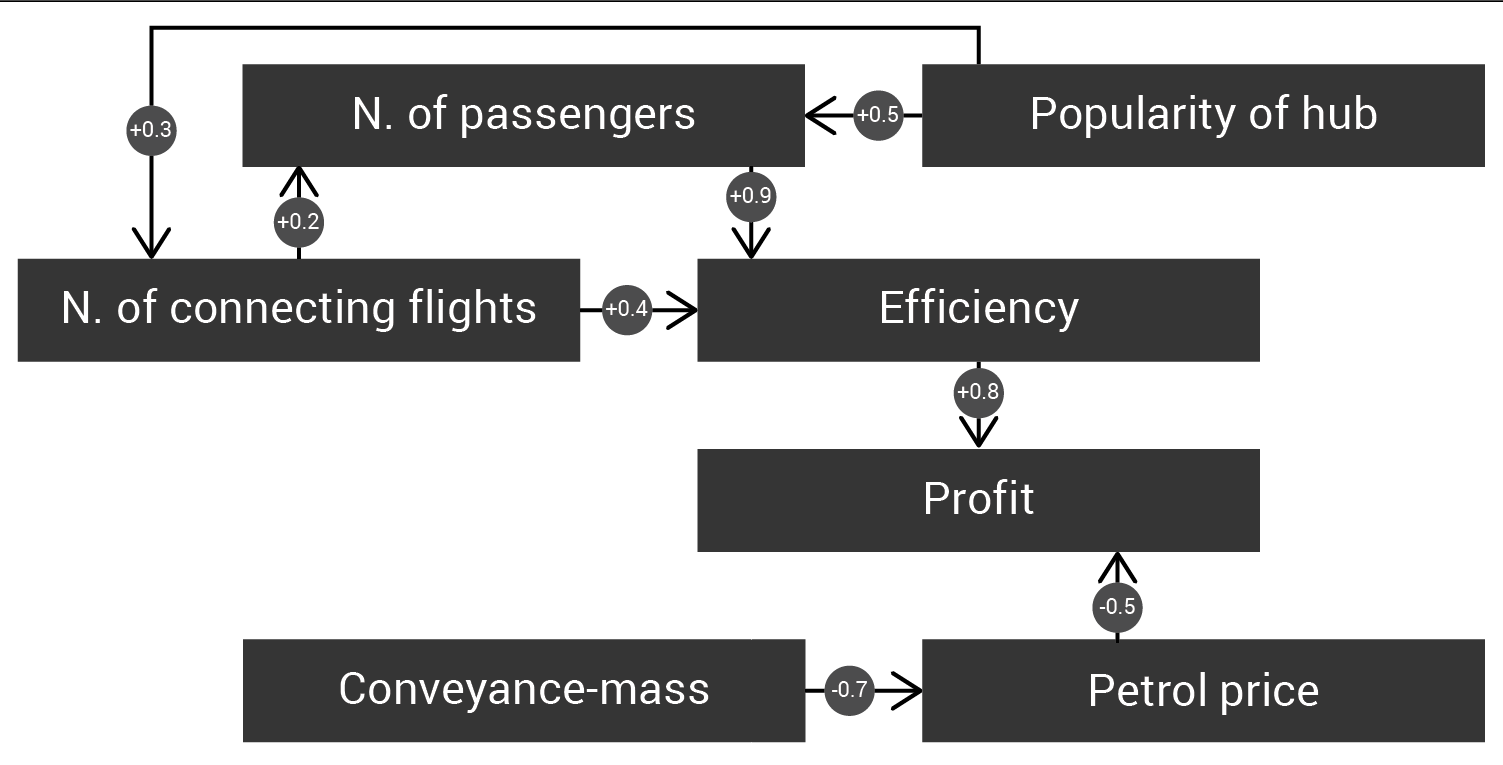
\includegraphics[width=3in]{img/ficFCM.png}
\caption{Influences of the profitability flight route A to B}
\label{fig:cm}
\end{figure}

FCM are widely used to represent a collection of knowledge of experts expressed by causal weighted digraphs. The developed model can be also interpreted by non field specific experts. This facilitates the transfer of knowledge in a simple, visual nature. If enough field specific data is available, FCM can be developed directly on this data and verified by field specific experts. That allows FCM to model complex problems based on large amounts of data and reduce it to the essential causal dependencies. This becomes more and more a useful property, since the global available amounts of data are growing increasingly in our days.\\
Developed FCM's can be used to \emph{explain} a complex system by showing degrees of causal influences of for the system relevant concepts. They can \emph{predict} how changes of these causal influences can affect other concepts or the system as whole. They are helping decision makers to \emph{reflect} over a given situation and see where adjustments are needed, this can be also influence the \emph{strategical planning}. Finally they can \emph{visualize} a complex system by introducing a graphical interface \cite{papageorgiou2013}.

\subsubsection{Formal Definition of FCM}
A FCM \begin{math} F = [-1,1] \end{math} is a 4-tuple \begin{math} (N,E,C,f) \end{math}, where
\begin{enumerate}
\item \begin{math} N = {N_{1},N_{2},...,N_{n}} \end{math} is a set of n concepts.
\item \begin{math} E: (N_{i},N_{j}) \rightarrow e_{ij} \end{math} is a function of \begin{math} N \times N \end{math} to \begin{math} K \end{math} associating \begin{math} e_{ij} \end{math} equal to zero if \begin{math} i = j \end{math}. Thus \begin{math} E(N \times N) = (e_{ij}) \in K^{n \times n} \end{math} is a connection matrix.
\item \begin{math} C: N_{i} \rightarrow C_{i} \end{math} is a function that at each concept \begin{math} N_{i} \end{math} associates the sequence of its activation degrees such as for \begin{math} t \in \mathbb{N}, C_{i}(t) \in L \end{math} given its activation degree at the moment \begin{math} t \end{math}. \begin{math} C(0) \in L^{n} \end{math} indicates the initial vector and specifies initial values of all concept nodes and \begin{math} C(t) \in L^{n} \end{math} is a state vector at certain iteration \begin{math} t \end{math}.
\item \begin{math} f: \mathbb{R} \rightarrow L \end{math} is a transformation function, which includes recurring relationship on \begin{math} t \geqslant 0 \end{math} between \begin{math} C(t+1) \end{math} and \begin{math} C(t) \end{math}.
\end{enumerate}
with \begin{math} \mathbb{R} \end{math} as a the set of real numbers and \begin{math} \mathbb{N} \end{math} denotes the set of natural numbers. \begin{math} K = [-1,1] \end{math} and \begin{math} L = [0,1] \end{math} \cite{stach2005}

The initiation of FCM starts with a initial vector, as input in a functional model(\ref{eq:fm}- \cite{stach2005}), this results in (initial) state vector. If over several iterations the sequence of state vectors is repeating, a steady state is reached.  
\begin{equation}\label{eq:fm}
\forall i \in \{1,...,n\},C_{i}(t+1) = f  \bigg(\sum_{i=1 \atop i \neq j}^{n} e_{ji}C_{j}(t)\bigg)
\end{equation}
The equation shows the multiplication of the initial vector with the corresponding weights. By applying a tranformation function, these weights can be normalized in the range of -1 to 1. To interpret a FCM in a first step, several indicators can be used (i.e. nodes can be classified into transmitter, receiver and ordinary, determined by the indegree and outdegree of each node \cite{ozesmi2004}). The centrality of a node can simply be measured by summing up the outdegree and indegree.

\subsection{Restriction Centered Theory}
\label{subsec:rct}
Fuzziness can be either expressed by using complex probabilistic models or, much simpler, a single word. \emph{"The flight lasts long"} is a statement of a person that may be grasped differently, even though there is a conjoint understanding about the concept of longevity. In brief, the RCT is seeking to evaluate the duration of a flight that is perceived as being long.

\subsubsection{General Idea of the RCT}
There are different concepts of defining a range of answers to a specific question (e.g. \emph{"How true is X?"}). The range can be defined either as a numerical interval, a set with predefined attributes or a probability distribution. What makes it complicated, is the fact that a word can be used in different contexts. And, even worse, depending on the context, the same word can have different meanings.\\
The main concept of the RCT is the restriction. It contains a higher variety in its range than an interval, a set or a probability distribution and combines all these concepts. Brief: a restriction's range contains every value that can be imagined. To illustrate the variety of possible answers, here an example: If a human is asked a question like \emph{"How profitable is the flight from A to B?"}, possible answers might be \emph{"It's 6.3 Billion US-Dollar per year"}, \emph{"It is more profitable than flight A to C"}, \emph{"It is not really profitable"}, \emph{"It is not as profitable as expected"}, and so on.\\
The first statement is palpably and can only be interpreted in one way. The other statements are referred by Zadeh \cite{zadeh2013} to as \emph{propositions}. Their outstanding property is the natural language. They contain fuzzy components, (i.e. a predicate as \emph{fast, loud, high}, a quantifier as \emph{many, less} and/or a probability as \emph{likely, eventually}). If a sentence includes a fuzzy predicate, the proposition is called zero-order, if it contains any one or more of the components, the sentence is called first-order fuzzy proposition.\\ 
A computing system asking how profitable the flight from A to B is, can interpret only the first answer, unless it is able to turn the proposition into a computable form. With the RCT, this is achievable.\\
To depict a proposition in a mathematical form, the Meaning Postulate (MP) is used:
\begin{equation} \label{eq:mp}
p \rightarrow X isr R
\end{equation}
In this equation, \begin{math} p \end{math} is the proposition that contains a variable to be restricted, \begin{math} X \end{math}, a restricting relation, \begin{math} R \end{math}, and the type of the restricting relation, \begin{math} r \end{math}. The better \begin{math} X \end{math}, \begin{math} R \end{math} and \begin{math} r \end{math} are mathematically defined, the better a restriction can be computed. Computations with restrictions look as pointed out in this example with fictive numbers: \emph{"One out of about 5 flights routes profitable. At Airline B, some 10 are profitable. What is the number of flights routes handled by Airline B?"} These two restrictions implicate that Airline B has 50 flight routes, even though there are more or less. Humans are used to deal with this kind of fuzzy reasoning. RCT offers the approach to solve these problems computationally.\\
A second important element of the RCT is the Canonical Form (CF). Basically, \begin{math} CF(p) \end{math} is the right-hand side part of Equation~\ref{eq:mp}, assigning the correct restriction type to the proposition.\\
The last concept is the Truth Postulate (TP). It computes the truth degree of a MP and is affiliated to the preciseness of the proposition. A truth degree can be phrased either numeric, (i.e. a first-order truth value), or in natural language, which is known as a second-order truth value \cite{zadeh2013}.
\subsubsection{Restrictions}
\label{subsubsec:restrictions}
Generally, natural language is used to express the restriction. The transformation of linguistic content into a calculable shape, is called precisiation. An explanatory database (ED) with a collection of relations is used for the precisiation of the variables \begin{math} X \end{math} and \begin{math} R \end{math}, or the computation of the truth value of \begin{math} p \end{math}. The precisiated variables are called \begin{math} X^{*} \end{math}, \begin{math} R^{*} \end{math} and \begin{math}p^{*} \end{math}. Thus, \begin{math} X^{*}=f(ED) \end{math} and \begin{math} R^{*}=g(ED) \end{math}. The numerical truth value of \begin{math} p \end{math}, \begin{math}nt_{p} \end{math}, can be depicted as \begin{math} nt_{p}=tr(ED) \end{math}, where \begin{math} tr \end{math} is called the truth function.\\
A restriction is subdivided into types. The three main types are the possibilistic restriction, the probabilistic restriction and the Z-restriction, which is a combination of the two former types. The restriction is called singular if the type of the restricting relation, \begin{math} R \end{math}, is a singleton (e.g. \begin{math} X=5 \end{math}). Otherwise, it is called nonsingular. Furthermore, the restriction may be direct, (i.e. the restricted variable is \begin{math} X \end{math}), or indirect (i.e. the restricted variable is a function of \begin{math} X \end{math}).\\
In the possibilistic restriction, \begin{math} R \end{math} is a fuzzy set, \begin{math} A \end{math}, where \begin{math} X \end{math} belongs to. The membership degree of \begin{math} X \end{math} to \begin{math} A \end{math} is calculated with the membership function, \begin{math} \mu_{A} \end{math}, of a possibility distribution.\\
The probabilistic restriction allows a statement about the sureness of a proposition. It is calculated with a density function of \begin{math} X \end{math}. Applied to natural language sentences, this means that the sureness of \emph{"usually"} is higher than the one of \emph{"sometimes"}. Probabilistic restrictions rarely occur exclusively in natural language, they are rather combined with possibilistic propositions. This is called a Z-restriction \cite{zadeh2013}. It contains natural language propositions, e.g. \emph{"Maybe Flight A to B is profitable"}, where \emph{"profitable"} is possibilistic and \emph{"maybe"} probabilistic.\\
The notation of the CF is differing depending on the type of restriction. A possibilistic restriction is denoted as \begin{math} X is A \end{math}, where \begin{math} A \end{math} is the fuzzy set or relation. A probabilistic restriction is shown as \begin{math} X isp p \end{math}, where the first \begin{math} p \end{math} is the probability density function. The second \begin{math} p \end{math} stands for proposition in the MP. A Z-restriction is depicted as \begin{math} X iz Z \end{math}, \begin{math} Z \end{math} is the combination of possibilistic and probabilistic restrictions and is defined as \begin{math} Z: Prob(X is A) is B \end{math}.\\
By combining both concepts, FCM and RCT, it is possible to formulate the contents of the FCM in clear natural language sentences with the aid of the RCT. In the following Chapter, a framework will be presented to do so.

\section{Framework}
\label{sec:framework}
It is now shown how natural language can be turned into a computable input. If there exists a FCM with nodes, edges and their respective weights, the computable input is available, but cannot be interpreted by an unexperienced person. Goal of the framework is to build FCM on raw data in a specific domain and to convert the numerical input of this FCM into natural language with the aid of the RCT.\\
First of all it has to be state out how the RCT can make use of a FCM: The FCM is usually built based on experiences, whether the experts' thoughts and observations or another big amount of data. So, the FCM has to serve as the ED for the RCT, since it provides the data that is used to precisiate variables.\\
In order to build a sentence, grammatically, at least a subject and a predicate is required. As a subject, a certain node of the FCM can be utilized, regardless of any context. The predicate has to be defined by the user, depending on the statement that he wants to make.\\
After all, this is not very informative yet. Therefore, two further elements have to be added to a standard sentence: An object, where another node can be placed, as well as a descriptive word like an adjective or adverb. It is thinkable that the edge weight can be used for this purpose, since it gives an idea about the strength of a relationship between subject and object. Depending on the weight, a certain word is chosen to describe the content.\\
Here, the RCT comes into play. The choice of words is similar to a possibilistic restriction. Each word has a different membership function. The totality of word options should cover the whole range of edge weights. The membership degree of each eligible word has then to be evaluated and the maximum among them is to be chosen. If there are two or more words with the same membership degree, it has to be assumed that these words can be used similarly.\\
A different nature of statements can also be made based on key figures such as the outdegree or the centrality of a node. Also, the state of a node at a certain moment during a simulation bears instructive information.\\
The nature of statements is strongly depending on the content of the FCM. This context-dependency is what makes it very difficult to define, for example, clear sets of words that can be used for any purpose.\\
In the following chapter, a use case will be defined to prove the validity of the outlined framework.

\section{Use Case Swiss: FCM model to describe flight passenger flows}
\label{sec:usecase}
The following use case will investigate on the passenger flows of an airline. A FCM will be constructed based on connecting passengers (Section \ref{subsec:design}), and the result shall be interpreted by a tool called interpretation engine, or query engine (Section \ref{subsec:queryengine}), converting the output into natural language statements (Section \ref{subsec:verbalization}). Finally, the generated output will be validated by a company's expert (Section \ref{subsec:validation}).\\
The data for this use case was provided by Swiss (airline code: LX). It contains 1.371.280 passenger records from January 2013, all these passengers travelled with one or more flights operated by LX. Every record contains the following information: Origin and destination of the traveler's journey (in separate fields), departure and arrival of the segment, flight number (operator and number in separate fields) and the document number.\\
The following table contains the cities and their respective airport codes that are used in this Chapter:
\begin{center}
\begin{table}[h]
\begin{tabular}{l|l}
\textbf{Code} & \textbf{Airport}\\ \hline
BCN & Barcelona\\ \hline
BHX & Birmingham\\ \hline
BOM & Mumbai\\ \hline
BSL & Basel\\ \hline
CDG & Paris Charles de Gaulle\\ \hline
DAR & Dar es Salaam\\ \hline
GVA & Geneva\\ \hline
HAM & Hamburg\\ \hline
JFK & New York John F. Kennedy\\ \hline
LAX & Los Angeles\\ \hline
LHR & London Heathrow\\ \hline
LYS & Lyon\\ \hline
MAN & Manchester\\ \hline
NRT & Tokyo Narita\\ \hline
PMI & Palma de Mallorca\\ \hline
TLV & Tel Aviv\\ \hline
ZRH & Zurich\\
\end{tabular}
\caption{Airport codes and their respective cities}
\label{tab:airportcodes}
\end{table}
\end{center}

\subsection{Design of the FCM}
\label{subsec:design}
When designing a new FCM, the specifications of the nodes, the graphs and the properties have to be determined before importing the data. The nodes are depicted as routes. Hence, a connecting passenger from Los Angeles through Zurich to Paris would be depicted as a link from the node ZRH-LAX (Zurich to Los Angeles) to the node ZRH-CDG (Zurich to Paris), as shown in Figure \ref{fig:noderoute}. The intermediate airport is mentioned twice in the node. If an airline has more than only one main hub, it is important to be able to distinguish the routes between the hubs. With the route node specification, this is assured.\newline
\begin{figure}[h]

\includegraphics[width=3in]{img/route.png}
\centering
\caption{Specification of FCM Nodes as Routes}
\label{fig:noderoute}
\end{figure}
\newline A problem to be solved are people who connect from another airline to Swiss flights. In any case it is necessary to identify these passengers as external connectors, since their share on certain routes is substantial for the airline. If they are not identified they are just counted as regular, non-connection passengers, which is unacceptable. Therefore, they need to be aggregated in a specific node. Hence, any route not being in the network is eliminated and the passengers can be identified on the route.\\
Following these argumentations, a node will be created for every route being in the network of Swiss. Its name will be composed by the two airports, first the hub and then the destination. If no hub is involved, then the airports will be referred to in alphabetical order. A separate node for all routes outside of Swiss' network will be created. Its name is OA, which stands for Other Airline.\\
The specification of the graphs is straightforward: A graph has to be set if a passenger flies on two routes within the same journey. The graph points to the direction of travel.\\
The remaining thing to be specified are the properties of the FCM's elements. Nodes hold the information about their name, that is, the route. A description is added, where the route is mentioned in plain text. And, finally, the total number of passengers traveling on this route is provided. It includes all passengers, be it connecting or not. Graphs hold the information about the route where a passengers comes from and the one it is connecting to. Also, the number of passengers on the graph as well as the ratio between the number of connectors and the total number of passengers on the original route is provided.\\

\subsection{Query Engine}
\label{subsec:queryengine}
In order to interpret the FCM, a query engine has to be defined that generates sentences in natural language. These statements are delivering a deeper insight into the FCM and allow a simpler interpretation of the data. For the present use case, based on FCM developed by available dataset two different issues can be considered: 
\begin{itemize}
\item The frequency of connecting passengers between two specific routes in a directed sense
\item The frequency of connecting passengers on a specific route to any other.
\end{itemize}
A third issue, the frequency of connecting passengers to a specific route from any other one could not be analyzed with the present data.\\
It is to mention that the frequency of connecting passengers from one route to another in relation to the total number of passengers on the first route, is very low. There are 4.050 different connections between two routes, the median is at 0.2\%, and the 90\%-percentile is at 1.1\%. This means that most of the connections have a very low share, which is why it is important to have an accurate distinction on low shares, whereas the shares above 20\% can be described with very few different words.\\
The frequency of connection passengers from one route to any other is, of course, higher than the first one. Here, the median is at 25\% and the 90\%-percentile is at 43.4\%. Therefore, the range between 20\% and 100\% of connections shall be described with five different adjectives. The remaining range between 0\% and 20\% will be covered with nine different adjectives.\\
All of the adjectives are supposed to express the frequency of a connection and are herewith ordered according to the frequency: \emph{Never, seldom, rarely, occasionally, infrequently, sometimes, frequently, often, regularly, normally, usually, generally, hardly ever,} and \emph{always}. Each of these words has got a membership function that defines the word's degree of truth in relation to the share of connecting passengers (\ref{subsubsec:restrictions}). For the adjective \emph{rarely} this corresponds to:

\begin{equation}
f(rarely)= \begin{cases}
50x + 0.5 & \text{if } 0 \leqslant x < 0.01\\
1 & \text{if } 0.01 \leqslant x < 0.03\\
-50x + 2.5 & \text{if } 0.03 \leqslant x < 0.05
\end{cases}
\end{equation}

When building the sentence, the word with the maximum membership degree is chosen, since it matches best the meaning that needs to be given to the sentence. Words with equal degrees can be used synonymously.\\
The frame of the sentences has to be defined for both issues that are considered. For the first issue, passengers that connect between two specific routes in a directed sense, the frame will be: \newline \emph{"Passengers travelling from (a) to (b) [c] connect to (d)."} \newline In this sentence, \emph{(a)} is the starting point of the journey which is normally the ending point of the route node, since the hub is always mentioned in first position. Then, \emph{(b)} is the hub, in which the passengers connect to the next flight. \emph{[c]} signifies the adjective, describing the frequency of connections and, finally, \emph{(d)} represents the ending point of the connection.\\
The second issue that is considered in the use case, describes the frequency of connecting passengers from a specific route to any other route. Here, the frame will be: \newline \emph{"Passengers travelling on the route (a) [b] connect to another flight."} \newline Here, for simplicity reasons, only the route \emph{(a)} and the describing word \emph{[b]} are used. Thus, it is a more general statement about connecting passengers, but nevertheless, the importance for analysis is at least as big as for the first issue.

\subsection{Verbalization of the FCM}
\label{subsec:verbalization}
After having defined and created the FCM, some specific connecting combinations are investigated. The choice of connections should cover the whole variety of long and short haul combinations, as well as journeys through all the three hubs.\\
The first issue is the connection from New York (JFK) via Zurich (ZRH) to Tel Aviv (TLV). The rate of passengers connecting from ZRH-JFK to ZRH-TLV is 0.0298. Based on this value, the truth value is now calculated for every adjective. There are two words having a maximum truth value of 1, that is, rarely and occasionally. These words can be used synonymously, which means that one word can be picked randomly. The sentence to be built would then be: \newline \emph{"Passengers travelling from New York JFK to Zurich \textbf{occasionally} connect to Tel Aviv."} \newline The following ten sentences are generated in the same way:
\begin{enumerate}
\item Passengers travelling from Dar es Salaam to Zurich often connect to London Heathrow.
\item Passengers travelling from Palma de Mallorca to Geneva frequently connect to Zurich.
\item Passengers travelling with Other Airlines never connect to the route Zurich-Birmingham.
\item Passengers travelling from Barcelona to Zurich never connect to Tokyo.
\item Passengers travelling from Tokyo to Zurich infrequently connect to Barcelona.
\item Passengers travelling from Barcelona to Basel seldom connect to Hamburg.
\item Passengers travelling from Mumbai to Zurich rarely connect to Manchester.
\item Passengers travelling on the route Zurich-Lyon usually connect another flight.
\item Passengers travelling on the route Geneva-London Heathrow occasionally connect to another flight.
\item Passengers travelling on the route Zurich-London Heathrow frequently connect to another flight.
\end{enumerate}

\subsection{Validation of the Output}
\label{subsec:validation}
The validation of the sentences mentioned in the previous section is done by the Head of Channel Management at Swiss International Air Lines Ltd. He is very experienced in the analysis of revenue and passenger data, as he jointly led the development of the passenger revenue information system and later introduced the booking outlook revenue information system. In his present position in Channel Management he is basically dealing with prognostics and market behavior, which is however often based on the analysis of the current or recently past situation.\\
In his feedback, he brought up important points regarding the number and choice of adjectives. The seasonal factor is pointed out as an improvement potential, so if the tool is used in a productive environment, this has imperatively to be implemented. The pleasing part of the feedback is, that there are no doubts about the correctness of the statements with regards to content. This leads to the conclusion that this use case was successful to prove the feasibility of verbalizing circumstances of a FCM with the aid of RCT.

\section{Lessons learned}
\label{sec:lessons}
There were three main points in the user's feedback that need to be improved:
\begin{itemize}
\item The adjective \emph{never} should be replaced by \emph{do not}
\item The number of adjectives should be reduced
\item The adjective \emph{usually} should be replaced by a different, unspecified word
\end{itemize}
It is true that the word \emph{never} implies a certain finality, saying that passengers do not connect neither now nor in future between two routes. Therefore it makes sense to replace it by a word such as \emph{do not} which rather makes a statement about the content and does not imply anything for future periods.\\
In order to simplify business decisions, it makes sense to reduce the number of adjectives. Each word would then cause a specific decision to be made. However, the sense of the tool is supposed to depict a big spectrum of adjectives, and hence, the tool can be used for a pre-analysis pointing out fields where deeper analysis is necessary. The business decisions should then be taken based on these further analyses.\\
In a user's perception, the word \emph{usually} is based on a standard that is either fulfilled or not. Since this standard is varying on every route and possibly even in every month, he disadvises the usage of the adjective. The shares that are used for choosing the word are based on the share of connecting passengers on the original route. Hence, the rating basis is varying on every route by definition. But, it is true that the seasonal factor, which has a very high importance in airline industry, is not considered in the tool. Doing so would imply a heavily higher data load and a time related dimension, which was not acceptable for the present use case. A workaround would be to create a FCM for every single month and to compare the results with each other.

\section{Conclusion}
\label{sec:conclusion}
FCM are used in many different fields of application: Medicine \cite{georgopoulos2003}, Ecology \cite{ozesmi2004}, Economy \cite{carvalho2004}, IT Project Management \cite{rodriguez2007} and many more. The interpretation of the underlying FCM was preferentially done with If-Then sentences, where a premise leads to a specific result.\\
This kind of interpretation contradicts the concept of fuzziness fundamentally, even though it is possible to formulate the premise as \emph{"If something is true to 0.2, then..."}. But the basic idea of having concepts and measuring the degree of membership in a fuzzy way is complex, because every fuzzy membership has to be expressed in many different If-Then clauses. With the possibilistic distribution, the RCT provides an instrument that eases the allocation of fuzzy membership degrees to concepts.\\
With the chosen approach of turning FCM output into natural language with the aid of the RCT, the interpretation of the FCM is left to the experts who build the FCM. They are in lead to define the sentence framework, to precisiate the set of words that is used and to specify the associated membership functions. This bares on one hand the chance that the content is made understandable to a bigger community, on the other hand there is the risk, that some information are manipulated or withheld, be it by mistake or even on purpose.\\
In his paper, Hagiwara \cite{hagiwara1992} points out three major improvement fields of the common FCM: 
\begin{itemize}
\item The proportionality of a relationship between two concepts
\item The lack of time delays
\item The impossibility of representing multiple causality. 
\end{itemize}
Especially the first point is interesting when trying to depict customer behavior in relation to the price, which is usually not linear but elastic. It also shows that the full potential of this approach is not yet exploited by far.\\
The introduction of a time dimension on the FCM is to be investigated. This is basically a problem of data size, which is even intensified when combining it with the learning algorithms.\\
On the RCT side the translation of results from the automated pattern recognition into natural language is a field, where many questions are not yet answered, especially in terms of granularity. This would make it possible to evaluate a FCM on an aggregated level and then to infer statements about more detailed parts of the FCM.\\
When reading these perspectives, one has always to keep in mind, that a FCM (like every model) is an abstraction of the real world. The goal of an abstraction is to create a simplified picture of complex relations. Many of the above-mentioned ideas do not imply any reduction of complexity when modeling the data with nowadays' technology. Nevertheless, this should be understood as an inspiration and motivation for tomorrow's ambitions.

\section*{Acknowledgment}
The authors would like to thank Edi Wolfensberger, who checked the verbalized output of the FCM and gave precious feedback from a user's perspective.

\bibliographystyle{IEEEtran}
\bibliography{fuzzieee2016}

\end{document}


